%%%%%%%%%%%%%%%%%%%%%%%%%%%%%%%%%%%%%%%%%%%%%%%%%%%%%%%%%%%%%%%%%%%%%%%%%%%%%%%%

\begin{solution}
\begin{enumerate}
  \item Expand $f(x) = x^2(1-x) = x^2-x^3$.  We can compute the coefficients
        $(f,\psi_k)$ as
            \[ (f,\psi_k) = \int_0^1 x^2 \big(\sqrt{2}\sin(k\pi x)\big)\, dx
                          - \int_0^1 x^3 \big(\sqrt{2}\sin(k\pi x)\big)\, dx.\]
        The first integral on the right can be computed using Mathematica, etc.
        Alternatively, one can work it out directly:
         \begin{eqnarray*}
              \sqrt{2} \int_0^1 x^2 \sin(k\pi x)\,dx
                         &=& \sqrt{2}\bigg(\Big[{-x^2 \cos{k\pi x} \over k\pi}\Big]_0^1
                                 + {2\over k\pi} \int_0^1 x\cos(k\pi x)\, dx\bigg) \\[0.5em]
                         &=& \sqrt{2}\bigg({(-1)^{k+1} \over k\pi}
                                 + {2\over k\pi} \int_0^1 x \cos(k\pi x)\, dx\bigg) \\[0.5em]
                         &=& \sqrt{2}\bigg({(-1)^{k+1} \over k\pi}
                        + {2\over k^2\pi^2} \Big[x\sin(k\pi x)\Big]_0^1
                                 - \int_0^1 \sin(k\pi x)\, dx\bigg) \\[0.5em]
                         &=& \sqrt{2}\bigg({(-1)^{k+1} \over k\pi}
                        - {2\over k^2\pi^2} \int_0^1 \sin(k\pi x)\, dx\bigg) \\[0.5em]
                         &=& \sqrt{2}\bigg({(-1)^{k+1} \over k\pi}
                        + {2\over k^3\pi^3}  \big[\cos(k\pi x)\big]_0^1\bigg) \\[0.5em]
                         &=& \sqrt{2}\Big({(2-k^2\pi^2)(-1)^k - 2 \over k^3 \pi^3}\Big).
         \end{eqnarray*}
        The second integral follows from integrating thrice by parts:
             \[ \int_0^1 x^3 \big(\sqrt{2}\sin(k\pi x)\big)\, dx
                  = {\sqrt{2}(-1)^n (6-k^2 \pi^2) \over k^3 \pi^3}.\]
        Assembling these results, we simplify to obtain
           \[ (f,\psi_k) = {\sqrt{2} \big(4(-1)^{k+1}-2\big) \over k^3\pi^3}.\]

         \begin{eqnarray*}
              \sqrt{2} \int_0^1 x^2 \sin(k\pi x)\,dx 
                         &=& \sqrt{2}\bigg(\Big[{-x^2 \cos{k\pi x} \over k\pi}\Big]_0^1
                                 + {2\over k\pi} \int_0^1 x\cos(k\pi x)\, dx\bigg) \\[0.5em]
                         &=& \sqrt{2}\bigg({(-1)^{k+1} \over k\pi}
                                 + {2\over k\pi} \int_0^1 x \cos(k\pi x)\, dx\bigg) \\[0.5em] 
                         &=& \sqrt{2}\bigg({(-1)^{k+1} \over k\pi}
                        + {2\over k^2\pi^2} \Big[x\sin(k\pi x)\Big]_0^1
                                 - \int_0^1 \sin(k\pi x)\, dx\bigg) \\[0.5em]
                         &=& \sqrt{2}\bigg({(-1)^{k+1} \over k\pi}
                        - {2\over k^2\pi^2} \int_0^1 \sin(k\pi x)\, dx\bigg) \\[0.5em]
                         &=& \sqrt{2}\bigg({(-1)^{k+1} \over k\pi}
                        + {2\over k^3\pi^3}  \big[\cos(k\pi x)\big]_0^1\bigg) \\[0.5em]
                         &=& \sqrt{2}\Big({(2-k^2\pi^2)(-1)^k - 2 \over k^3 \pi^3}\Big).
         \end{eqnarray*} 

    \item Partial sums of the series formula for $f$ are shown in the plots below.
          Code follows at the end of the problem.  The function $f$ happens to 
          satisfy homogeneous Dirichlet boundary conditions, and convergence is
          quite quick.
          \begin{center}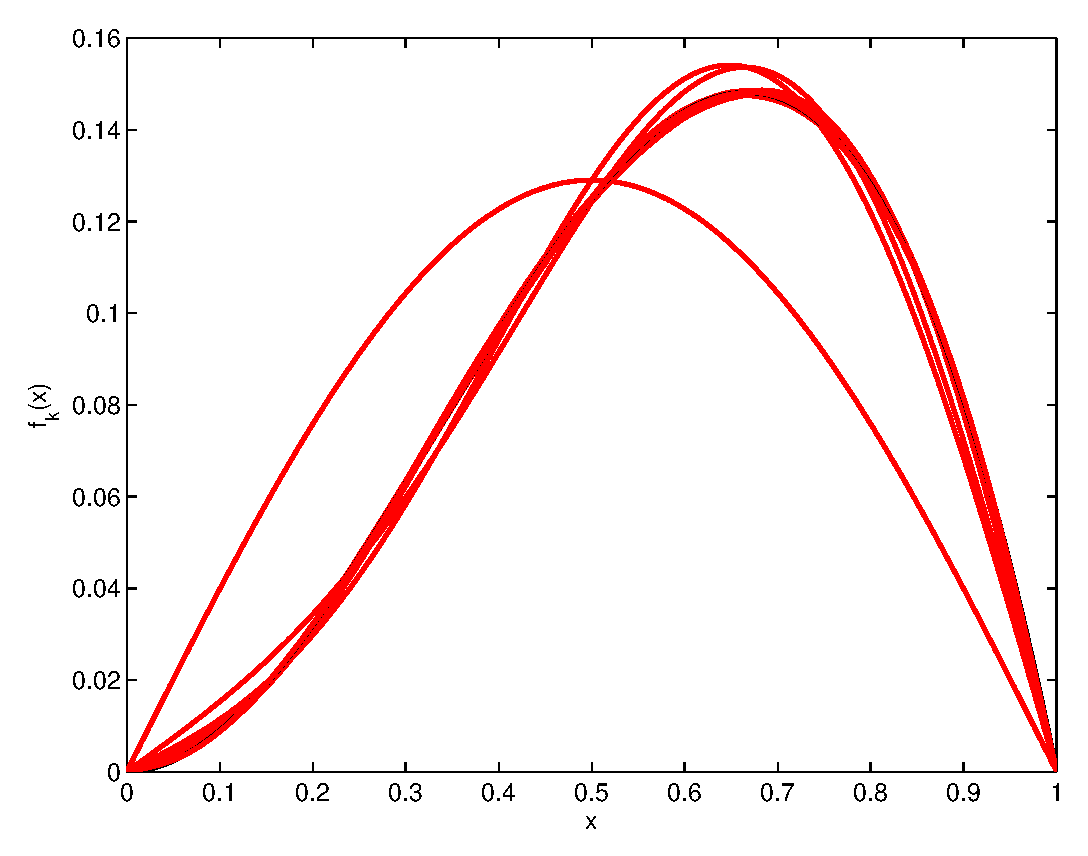
\includegraphics[scale=0.45]{sineseries2b}\end{center}
          \begin{center}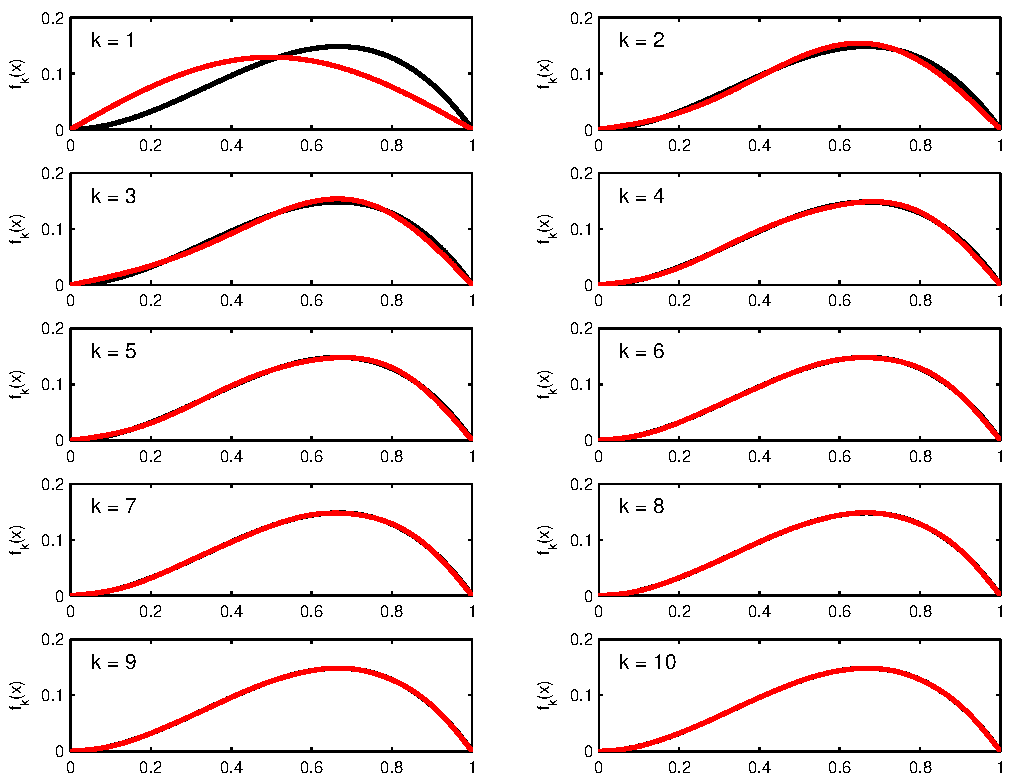
\includegraphics[scale=0.7]{sineseries2c}\end{center}
         
    \vspace*{1em} 
    \item The true solution to this problem (not asked for in the problem statement)
          can be computed as $u(x) = (2x-5x^4+3x^5)/60$.
          The spectral method gives $u(x)$ as the series
               \[ u(x) = \sum_{k=1}^\infty \sqrt{2}\Big({4(-1)^{k+1}-2 \over k^5 \pi^5}\Big)
                          \big(\sqrt{2} \sin(k \pi x)\big), \]
          whose coefficients decay even more rapidly than did the coefficients
          for $f$ itself, explaining the fantastic convergence rate.
          The next two plots compare the sum from the spectral method (red lines)
          to the true solution (black line).  The following plot shows the error as
          a function of $x$ for $k=1,\ldots, N$.

          \begin{center}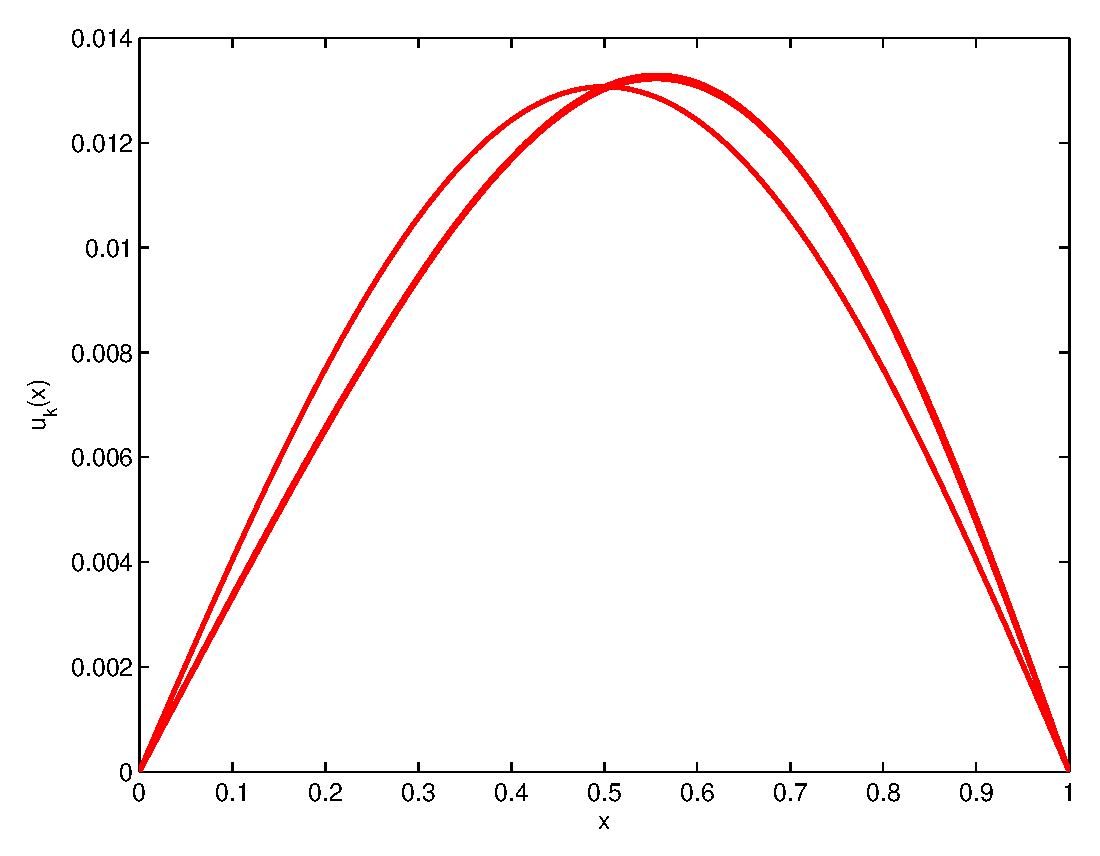
\includegraphics[scale=0.45]{sineseries2d}\end{center}
          \begin{center}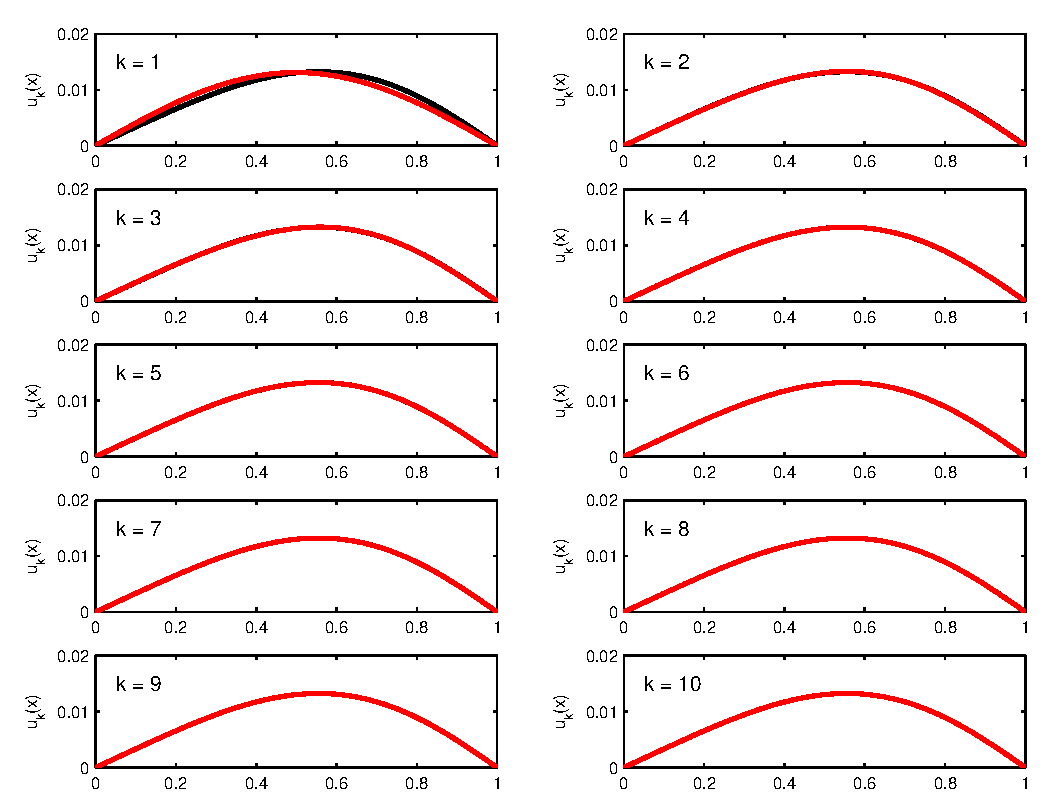
\includegraphics[scale=0.7]{sineseries2e}\end{center}

          Plots of the error as $k$ increases:
          \begin{center}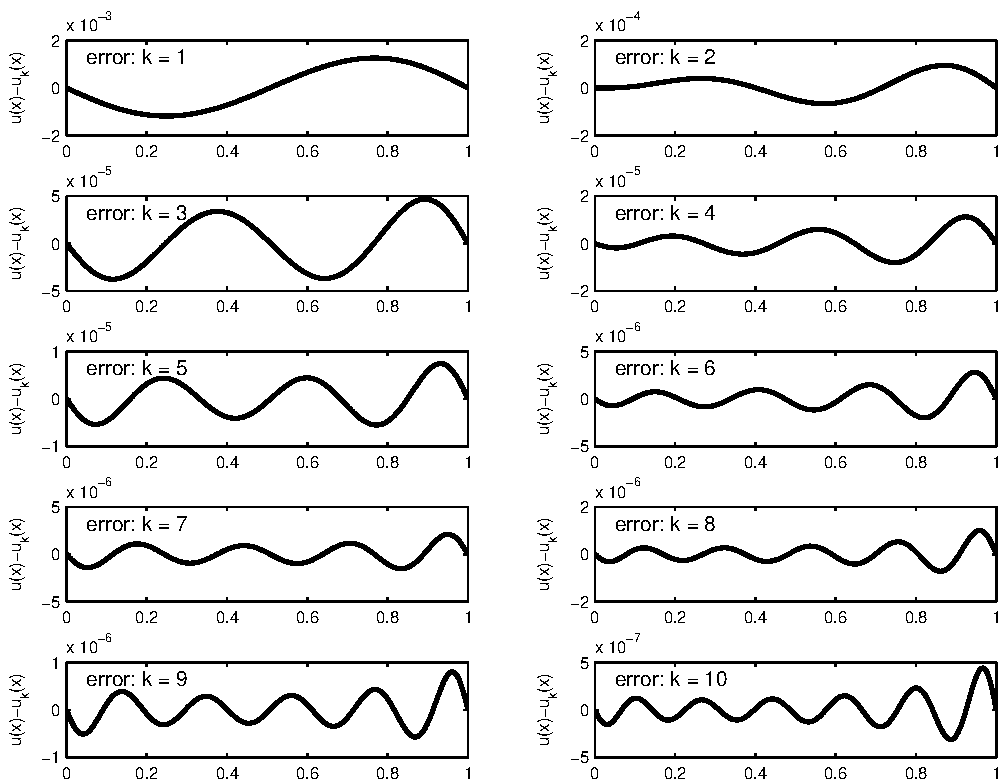
\includegraphics[scale=0.7]{sineseries2f}\end{center}

\item To incorporate inhomogeneous Dirichlet boundary conditions, we will write the 
       solution in the form $u = \widehat{u} + w$, where the correction
       $w(x) = \alpha + \beta x$ has the property that $-w''(x) = 0$, and 
       $\widehat{u}$ denotes the solution to $L\widehat{u} = f$ 
      with homogeneous Dirichlet boundary conditions; thus $\widehat{u}$ is precisely
      the solution $u$ worked out in part~(c).  
      Notice that $u(0) = w(0) = \widehat{u}(0) = w(0) = \alpha$ and 
      $u(1) = w(1) = \widehat{u}(1) = w(1) = \alpha+\beta$.
      Since we want $u(0) = -1/100$ and $u(1) = 1/100$, we solve to find:
         \[ \alpha = -1/100, \qquad \beta = 2/100.\]
      Thus, the solution to our equation with these inhomogeneous boundary conditions is:
               \[ u(x) = -1/100 + (2/100) x 
                        + \sum_{k=1}^\infty \sqrt{2}\Big({4(-1)^{k+1}-2 \over k^5 \pi^5}\Big)
                          \big(\sqrt{2} \sin(k \pi x)\big), \]
      The plot of $u_{10}(x) = w(x) + \widehat{u}_{10}(x)$ is shown below.
\begin{center}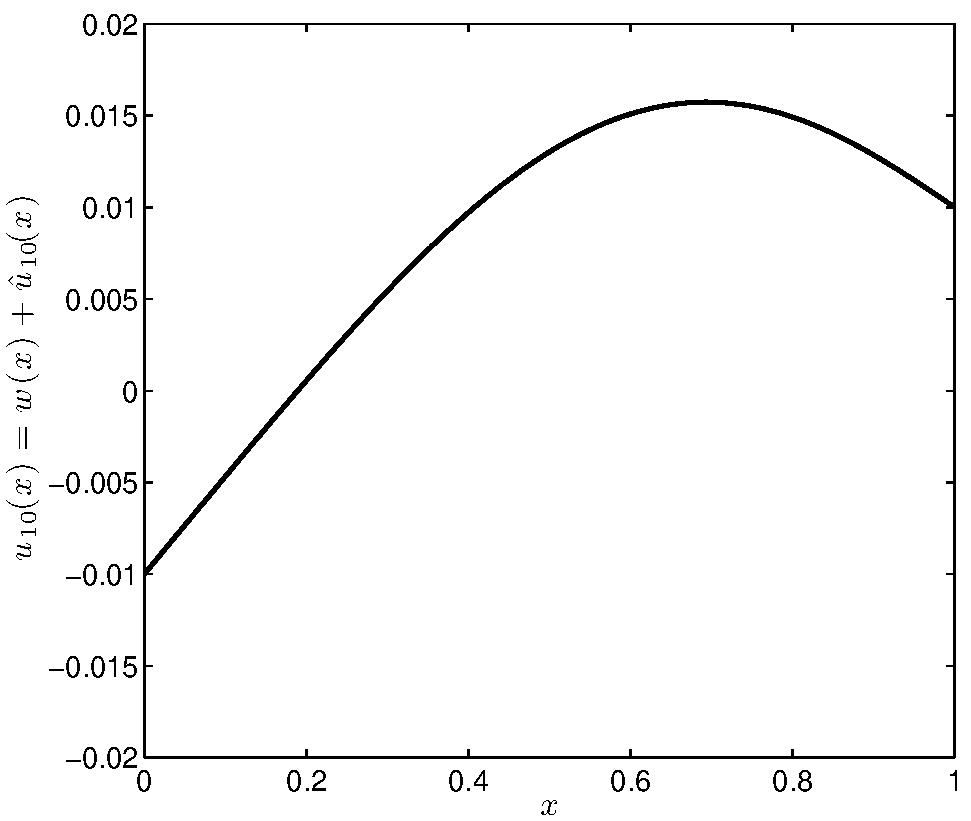
\includegraphics[scale=0.7]{sineseries2g}\end{center}
\end{enumerate}

The plots above were computed using the following MATLAB code.

{\small \begin{verbatim}
% f(x) = x^2(1-x);

% compute the inner products (f, phi_k) for k=1,...,30
  k = [1:30]';
  ck = sqrt(2)*(4*(-1).^(k+1)-2)./(k.^3*pi^3);

% plot first 10 partial sums fk, all on one plot
 figure(2), clf
 x = linspace(0,1,500)';
 fk = zeros(size(x));
 for k=1:10
    plot(x,(x.^2).*(1-x),'k-','linewidth',2), hold on
    fk = fk + ck(k)*sqrt(2)*sin(k*pi*x);
    plot(x,fk,'r-','linewidth',2)
    xlabel('x'), ylabel('f_k(x)')
 end
 print -depsc2 sineseries2b

% plot first 10 partial sums fk, all on 10 different plot
 figure(3), clf
 x = linspace(0,1,500)';
 fk = zeros(size(x));
 for k=1:10
    subplot(5,2,k)
    plot(x,(x.^2).*(1-x),'k-','linewidth',2), hold on
    fk = fk + ck(k)*sqrt(2)*sin(k*pi*x);
    plot(x,fk,'r-','linewidth',2)
    axis([0 1 0 0.2])
    set(gca,'fontsize',8)
    text(0.05,0.16,sprintf('k = %d',k))
    ylabel('f_k(x)')
 end
 print -depsc2 sineseries2c


% plot first 10 partial sums uk, all on one plot
 figure(4), clf
 x = linspace(0,1,500)';
 uk = zeros(size(x));
 for k=1:10
    plot(x,(2*x-5*(x.^4)+3*(x.^5))/60,'k-','linewidth',2), hold on
    lamk = k^2*pi^2;
    uk = uk + ck(k)/lamk*sqrt(2)*sin(k*pi*x);
    plot(x,uk,'r-','linewidth',2)
    xlabel('x'), ylabel('u_k(x)')
 end
 print -depsc2 sineseries2d

% plot first 10 partial sums uk, all on 10 different plot
 figure(5), clf
 x = linspace(0,1,500)';
 uk = zeros(size(x));
 for k=1:10
    subplot(5,2,k)
    plot(x,(2*x-5*(x.^4)+3*(x.^5))/60,'k-','linewidth',2), hold on
    lamk = k^2*pi^2;
    uk = uk + ck(k)/lamk*sqrt(2)*sin(k*pi*x);
    plot(x,uk,'r-','linewidth',2)
    axis([0 1 0 .02])
    set(gca,'fontsize',8)
    text(0.05,0.015,sprintf('k = %d',k))
    ylabel('u_k(x)')
 end
 print -depsc2 sineseries2e

% plot error in first 10 partial sums uk, all on 10 different plot
 figure(6), clf
 x = linspace(0,1,500)';
 uk = zeros(size(x));
 for k=1:10
    subplot(5,2,k)
    lamk = k^2*pi^2;
    uk = uk + ck(k)/lamk*sqrt(2)*sin(k*pi*x);
    plot(x,(2*x-5*(x.^4)+3*(x.^5))/60 - uk,'k-','linewidth',2), hold on
    set(gca,'fontsize',8)
    text(0.05,max(ylim)-.175*diff(ylim),sprintf('error: k = %d',k))
    ylabel('u(x)-u_k(x)')
 end
 print -depsc2 sineseries2f

% inhomogeneous boundary condition:
% plot first 10 partial sums uk, all on 10 different plot
 figure(7), clf
 x = linspace(0,1,500)';
 w = -1/100 + (2/100)*x;
 uhatk = zeros(size(x));
 for k=1:10
    lamk = k^2*pi^2;
    uhatk = uhatk + ck(k)/lamk*sqrt(2)*sin(k*pi*x);
    plot(x,w+uhatk,'k-','linewidth',2)
    axis([0 1 -.02 .02])
    set(gca,'fontsize',14)
    ylabel('$u_{10}(x) = w(x) + \hat{u}_{10}(x)$','fontsize',16,'interpreter','latex')
    xlabel('$x$','fontsize',16,'interpreter','latex')
 end
 print -depsc2 sineseries2g
\end{verbatim}}

\end{solution}

